\section{Program memory layout} \label{Memory Layout}

This section explores how a C Program is laid out in memory. We will use the GNU C Compiler memory layout as the template. Each operating system and C compiler combination may have slightly different naming conventions but the underlying principles remain the same.
 \begin{figure}[H]
\centerline{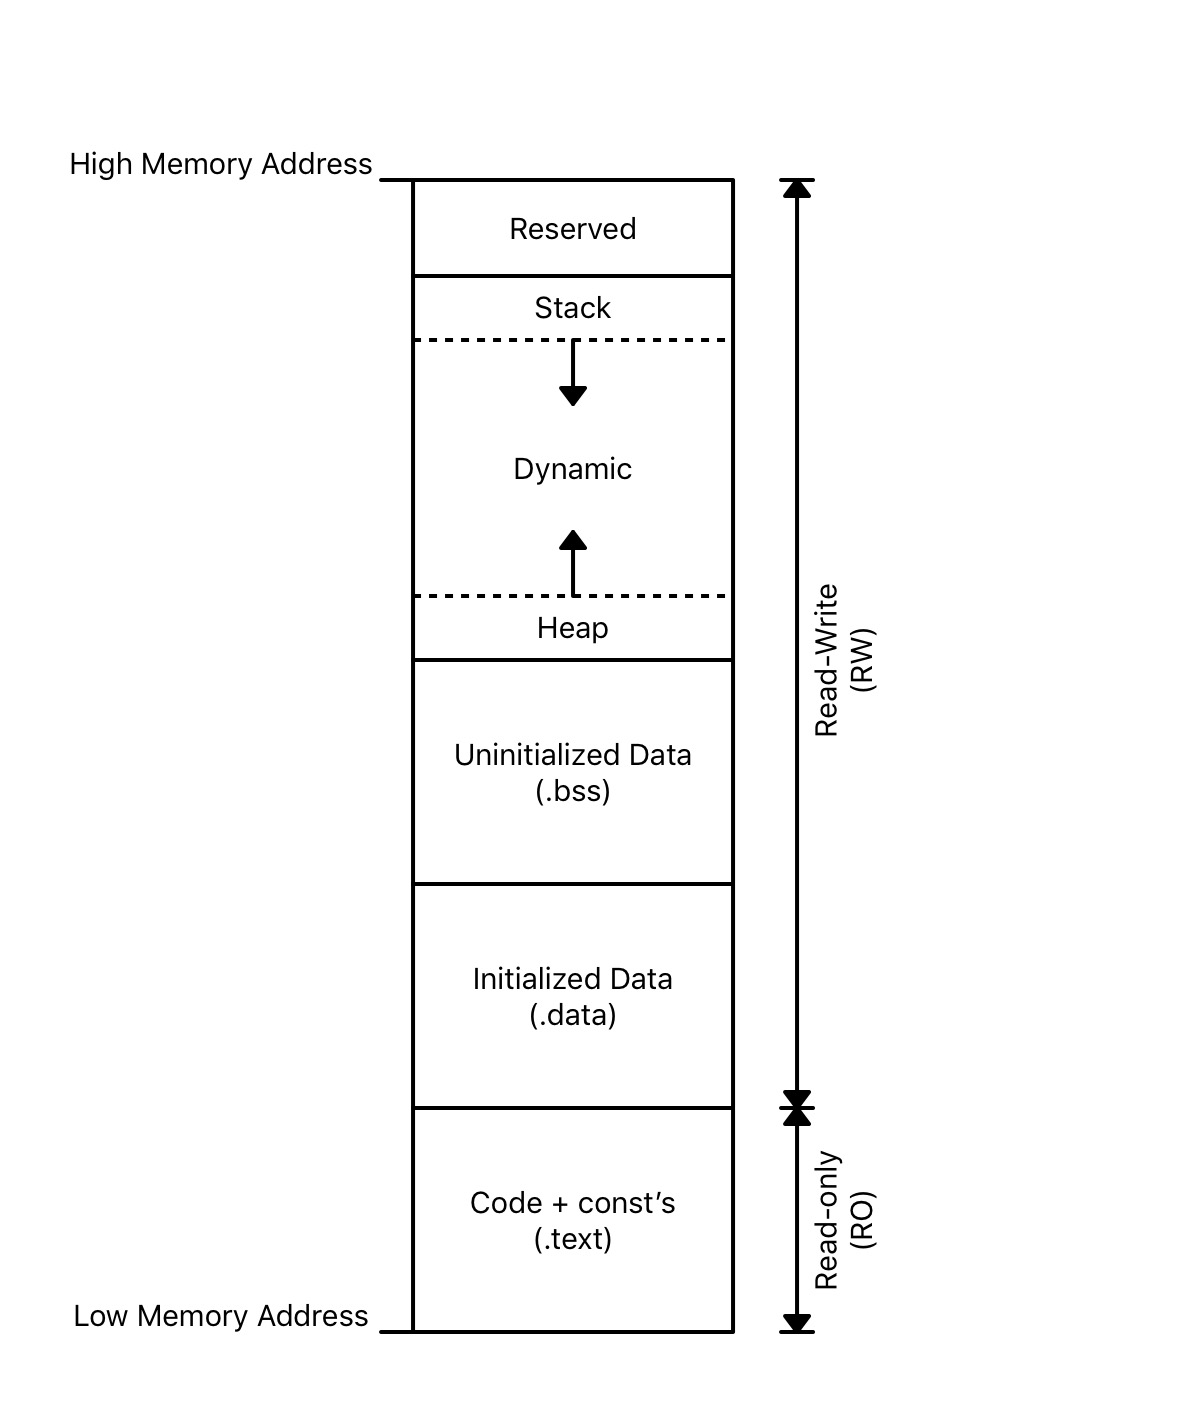
\includegraphics[width=0.6\textwidth]{layout.jpg}}
\caption{C Program Memory Layout}
\label{CProgMem}
\end{figure}

For simplicity we will just explore a single threaded C program, as shown in figure \ref{CProgMem}. A program is divided into a number of memory segments i.e. \textit{.text}, \textit{.data}, \textit{.bss} and finally the \textit{dynamic} and \textit{reserved} areas. For a multi-threaded program there will be a stack dedicated to each thread within the dynamic area. 

When compiling and linking for an embedded system it is important control where individual segments are physically located. For some systems the segments may not be contiguous and in fact may be purposely placed in specific memory types. These types may have different read-write attributes, size capacity, longevity or even power characteristics.    

Note, figure \ref{CProgMem} has low memory addresses at the bottom ascending to higher memory addresses at the top. For a reminder about variable types recommend going back to section \ref{avari}.

\newpage

\begin{lstlisting}[language=C,showstringspaces=false,caption={Image segment breakdown},captionpos=b,label=filesize]
 1 $ size calling.o
 2  text	   data	    bss	    dec	    hex	filename
 3   196	      0	      0	    196	     c4	calling.o
 4 $ 
\end{lstlisting}

Listing \ref{filesize} shows the breakdown of a object file \textit{calling.o}. The listing shows that the object only contains instruction code (text) and no initialized (data) nor uninitialized (bss) data. This information is extracted using the GNU compiler utility tool \textit{size}. 

\subsection{.text segment} \index{.text}

\textit{.text} memory segment is a fixed size non-modified memory area that contains the executable instructions (and the \textit{const} variables) of a C program. The size is determined by the compiled source code. It is a read-only segment since neither the instructions nor the \textit{const} variables should be modified during the lifetime of the program. 

The read-only attribute means that this segment can be placed (and executed) in nonvolatile memory. This can be important when dealing with embedded systems. Especially if the volatile memory is limited in size.

\subsection{.data segment} \label{.data} \index{.data}

\textit{.data} memory segment is a fixed size and contains the initialized data (e.g. \textit{x=42;}). The data represents global or static variables which have been set a value and can be modified. The number of variables determines the size of the segment. For deeply embedded systems it is common for the \textit{.data} segment to first reside in non-volatile memory. During the program startup initiation the \textit{.data} segment is copied from non-volatile memory to some form of volatile memory. The volatile memory allows the data to be modified during program execution.

\subsection{.bss segment} \index{.bss}

\textit{.bss} memory segment is a fixed size and contains uninitialized data. The data is a combination of global and static variables which are not initialized to a specific value by the program (e.g. \textit{static int x;}). The number of variables determines the size of the segment. For this reason variables are initially set to the value zero. This is normally achieved programmatically using a loop to set the variables to zero.

Similar to \textit{.data} segment, in section \ref{.data}, the \textit{.bss} segment is held in volatile memory because these variables may change in value as the program executes.

\subsection{Dynamic area}

Dynamic segment is the part of the memory layout that grows and shrinks depending upon usage. The size limit remains constant. Contrary to \textit{.text}, \textit{.data} and \textit{.bss} segments which remain fixed size throughout the lifetime of the program. The dynamic segment contains both the \textit{C User Stack} and the \textit{Heap} which are continuously growing and shrinking during program execution.

\subsubsection{Program stack}

The program stack is used during calculations, preserving data, restoring data and calling functions. Each hardware architecture has a unique way to call functions and return values. This is normally standardized in a document called the \textit{Procedure Call Standard} (PCS), explained in more detail in section \ref{callingass}. The PCS defines how parameters are passed into a function and how the return values are stored. For many architectures the first n-parameters are passed in as registers and all subsequent parameters are held on the stack. These parameters are held on program stack. Also the function return address can also be held on the stack.  

\subsubsection{Heap}

The \textit{heap} is the area where dynamic memory is stored and removed. It competes with the same for memory as the stack. For more details on \textit{Dynamic Memory Allocation} see section \ref{DynamicMem}.

For embedded systems the heap may be used during the initialization phase but after that point the heap will remain fixed in size i.e. it neither grows nor shrinks. This is because dynamic memory is difficult in control in systems where high reliability is required.

\subsection{Reserved area}

This area of memory is reserved for command line inputs and environment details when the C program is called.
